\documentclass[ASNA]{USG} %twocolumn
\usepackage{anyfontsize} %

\usepackage{colortbl}   % For coloring table lines
\usepackage{xcolor}     % For color definitions

\usepackage{steinmetz}



\graphicspath{{./images/}}
\specialissue{Campus-DDoS-SDN: Multi-vector DDoS detection in software-defined campus networks}

\articletype{ORIGINAL ARTICLE}%
\subarticletype{Software-defined networking and security}

\received{25 November 2026}
\revised{25 November 2026}
\accepted{25 November 2026}
\journal{Journal of Computer Networks and Communications}
\volume{0}
\copyyear{2026}
\startpage{1}
\articledoi{10.1002/0000}

%\raggedbottom

%%
%\renewcommand\ShowFrameLinethickness{0.15pt}
%\renewcommand*\ShowFrameColor{\color{red}}


\begin{document}
\title{Campus-DDoS-SDN: Multi-vector DDoS detection in software-defined campus networks}
%\subtitle{Subtitle}
\transtitle{Campus-DDoS-SDN: Multi-vector DDoS detection in software-defined campus networks}
\subtranstitle{trans-subtitle}
\author[1]{Cristhian M. Casas}[https://orcid.org/0009-0000-9070-9010][\linkedin{https://www.linkedin.com}]
\author[2]{Alessandro P. Martínez}[][\linkedin{https://www.linkedin.com}]
\author[3]{Anna C. Leiva}[https://orcid.org/0009-0003-2087-2148][\linkedin{https://www.linkedin.com}]
\author[4]{Ricardo L. Lozano}[https://orcid.org/0000-0001-7037-2721][\linkedin{https://www.linkedin.com/in/ricardollanoslozano/}]
\author[5]{Jaime S. Terrel}[https://orcid.org/0000-0002-0285-0899]
\author[6]{Henry M. Quispe}[https://orcid.org/0000-0003-3055-9166]


%\author[6]{Alexis Conway}[https://orcid.org/0000-0001-7037-2721]

%\author[7]{Uttara Chakraborty}[https://orcid.org/0000-0001-7037-2721]

%\author[8]{Kathleen T. Daniels}[https://orcid.org/0000-0001-7037-2721]

%\author[9]{Gelo de la Cruz}[https://orcid.org/0000-0001-7037-2721]

%\author[10]{Laura Ferrer-Font}[https://orcid.org/0000-0001-7037-2721]

%\author[11]{Andrew Filby}[https://orcid.org/0000-0001-7037-2721]

%\author[12]{David M. Gravano}[https://orcid.org/0000-0001-7037-2721]

%\author[13]{Michael D. Gregory}[https://orcid.org/0000-0001-7037-2721]

%\author[14]{Christopher Hall}[https://orcid.org/0000-0001-7037-2721]

%\author[15]{Christian Kukat}[https://orcid.org/0000-0001-7037-2721]

%\author[16]{André Mozes}[https://orcid.org/0000-0001-7037-2721]

%\author[17]{Diana Ordoñez-Rueda}[https://orcid.org/0000-0001-7037-2721]

%\author[18]{Eva Orlowski-Oliver}[https://orcid.org/0000-0001-7037-2721]

%\author[19]{Isabella Pesce}[https://orcid.org/0000-0001-7037-2721]

%\author[20]{Ziv Porat}[https://orcid.org/0000-0001-7037-2721]

%\author[21]{Nicole J. Poulton}[https://orcid.org/0000-0001-7037-2721]

%\author[22]{Kristen M. Reifel}[https://orcid.org/0000-0001-7037-2721]

%\author[23]{Aja M. Rieger}[https://orcid.org/0000-0001-7037-2721]

%\author[24]{Rachael T. C. Sheridan}[https://orcid.org/0000-0001-7037-2721]

%\author[25]{Gert Van Isterdael}[https://orcid.org/0000-0001-7037-2721]

%\author[14]{Rachael V. Walker}[https://orcid.org/0000-0001-7037-2721]

\authormark{Martínez \textsc{et al.}}
\titlemark{Campus-DDoS-SDN: A Python-based testbed for multi-vector DDoS attack detection in software-defined campus networks}

\address[1]{\orgdiv{Facultad de Ingeniería de Sistemas, }\orgname{Universidad Nacional del Centro del Perú, }%
\orgaddress{\state{Huancayo, }\country{Perú}}}

\address[2]{\orgdiv{Facultad de Ingeniería de Sistemas, }\orgname{Universidad Nacional del Centro del Perú, }%
\orgaddress{\state{Huancayo, }\country{Perú}}}

\address[3]{\orgdiv{Facultad de Ingeniería de Sistemas, }\orgname{Universidad Nacional del Centro del Perú, }%
\orgaddress{\state{Huancayo, }\country{Perú}}}

\address[4]{\orgdiv{Facultad de Ingeniería de Sistemas, }\orgname{Universidad Nacional del Centro del Perú, }%
\orgaddress{\state{Huancayo, }\country{Perú}}}

\address[5]{\orgdiv{Facultad de Ingeniería de Sistemas, }\orgname{Universidad Nacional del Centro del Perú, }%
\orgaddress{\state{Huancayo, }\country{Perú}}}

% Falta
\corres{Cristhian M. Casas  (\email{cristhianmartinezcasas@gmail.com}) ~|~ Ricardo L. Lozano (\email{llanoslozano2005@gmail.com})}

\editor{\textbf{Academic Editor:}  ~|~ \textbf{Guest Editor:} }

 

\presentaddress{This work was produced in the context of SDN and DDoS detection research at the Universidad Nacional del Centro del Perú}

\fundingInfo{This research received no external funding.}

\keywords{Software-defined networking | machine learning | DDoS attack detection | Mininet | network traffic classification}

\transkeywords{Software-defined networking | machine learning | DDoS attack detection | Mininet | network traffic classification}

\newcommand{\Fmacro}{0{,}918~$\pm$~0{,}149}


\abstract[ABSTRACT]{Software-defined networks (SDN) are a common practice in enterprise IT management systems due to their simplified management and ease of use, but they also pose a latent risk: if compromised, they could compromise all services that depend on that network. Studies of this type of network typically use synthetic traffic, which undermines the value of the data because it does not accurately represent real traffic; or, alternatively, they include only a minimal number of attack vectors. This study addresses these challenges by, first, capturing real traffic at a public university using four attack vectors: TCP-SYN, HTTP, Slowloris, and ICMP, while simultaneously simulating DDoS attacks in a Dockerized environment that emulates the university’s SDN networks. Traffic classification was performed using three classification algorithms: Naive Bayes, Random Forest, and Logistic Regression. Traffic was captured in 120-second sessions for each SDN over five iterations, ultimately yielding 230,692 network packets. The results indicate that the classification methods yielded optimal results, with a minimum F1 score of 0.997 for logistic regression and 0.999 for both the Random Forest and Naive Bayes models.  The study achieves its objective by generating a multclass network traffic dataset and by establishing classification methods that can be fine-tuned using the proposed data.}

 \transabstract[transABSTRACT]{Software-defined networks (SDN) are a common practice in enterprise IT management systems due to their simplified management and ease of use, but they also pose a latent risk: if compromised, they could compromise all services that depend on that network. Studies of this type of network typically use synthetic traffic, which undermines the value of the data because it does not accurately represent real traffic; or, alternatively, they include only a minimal number of attack vectors. This study addresses these challenges by, first, capturing real traffic at a public university using four attack vectors: TCP-SYN, HTTP, Slowloris, and ICMP, while simultaneously simulating DDoS attacks in a Dockerized environment that emulates the university’s SDN networks. Traffic classification was performed using three classification algorithms: Naive Bayes, Random Forest, and Logistic Regression. Traffic was captured in 120-second sessions for each SDN over five iterations, ultimately yielding 230,692 network packets. The results indicate that the classification methods yielded optimal results, with a minimum F1 score of 0.997 for logistic regression and 0.999 for both the Random Forest and Naive Bayes models.  The study achieves its objective by generating a multclass network traffic dataset and by establishing classification methods that can be fine-tuned using the proposed data.}

\abbr{CICFlowMeter, OpenFlow, SDN, DDoS, HTTP, ICMP, SYN, Ryu, Mininet, ML.}




\contributed{All authors contributed to the design, implementation, validation and writing of the manuscript.}

  \dedicated{Dedicated to reproducible SDN research and applied network security education.}

\copyright{This is an open access article under the terms of the \href{Creative Commons Attribution-NonCommercial}{Creative Commons Attribution-NonCommercial} License, which permits use, distribution and reproduction in any medium, provided the
original~work~is~properly cited and is not used for commercial purposes.
\\[5pt]
  \textcopyright~2026 The Author(s) \textit{Journal of Computer Networks and Communications} published by Wiley Periodicals LLC on behalf of American Institute of Chemical Engineers.}

%\openaccessstatement

\maketitle
%\afterpage{\aftergroup\restoregeometry}

%\onecolumn

\section{Introduction}\label{sec:intro}

Software-defined networking (SDN) decouples the control plane from the data plane, concentrating network intelligence in a logically centralized controller \citep{kreutz2015sdn}. This centralization simplifies network management, but it also turns the controller into a single point of failure: a distributed denial-of-service (DDoS) attack that saturates the controller, the switches, or a hosted service can degrade or take down the entire network segment it governs. Detecting such attacks early, and separating them reliably from legitimate traffic spikes, requires datasets that are both representative of real SDN deployments and precisely labelled.

Most publicly available intrusion-detection datasets, such as NSL-KDD \citep{tavallaee2009nslkdd}, CICIDS2017 \citep{sharafaldin2018cicflowmeter}, and CICDDoS2019 \citep{sharafaldin2019cicddos2019}, were not captured inside an SDN environment: they lack OpenFlow-specific signals, such as flow-table occupancy or controller load, and are nonetheless often reused out of context to train SDN-targeted classifiers. Recent work has started to close this gap by generating DDoS datasets directly inside Mininet/Ryu testbeds. Kumar and Gupta released two single-vector datasets built this way: a TCP-SYN flood dataset \citep{kumar2025synflood} and, more recently, an ICMP-flood dataset \citep{kumar2026icmpfloodsdn} in which normal traffic is captured by connecting a Mininet host to a live internet connection and browsing real websites (YouTube, Facebook, news, etc.), instead of relying on synthetic traffic generators. This real-traffic approach increases realism, but it introduces two practical limitations for a reusable benchmark: the resulting dataset is tied to a single attack vector, and it is not reproducible across runs, since the captured content and timing depend on whatever the live internet happens to serve at capture time.

This work, Campus-DDoS-SDN, addresses both limitations within a single, fully reproducible testbed. Four attack vectors (TCP-SYN flood, HTTP flood, Slowloris, and ICMP flood) are launched from already-compromised hosts against one shared victim, a web portal, inside a Mininet/Ryu topology that mimics a university campus: a core/DMZ switch layout plus one emulated laboratory per academic area. Unlike prior single-vector or fully-separated-capture datasets, legitimate users keep browsing the portal throughout every attack, so each capture mixes benign and malicious flows against the same target, as a real DDoS incident would. Ground-truth labels are assigned per source IP rather than per capture file, and every run additionally logs the attack's effect on the victim as perceived by a real client (HTTP response code, latency, active connections), alongside network-level indicators (packets and bytes per second) and OpenFlow controller telemetry collected by a custom Ryu application (flow-table statistics, per-source flow counts and source-IP entropy sampled at a fixed interval). The complete environment, including the traffic generators, the custom web portal, and the labelling pipeline, is packaged as a Docker image to remove any dependency on a live internet connection or on a specific host operating system.

The main contributions of this work are:

\begin{enumerate}[label=\roman*.]
  \item A multi-class DDoS dataset covering four attack vectors
        against a single victim inside a realistic, multi-segment SDN topology, instead of a single attack type against a flat
        network.

  \item Per-flow, per-source-IP labelling that keeps legitimate and
        malicious traffic mixed within the same capture, closer to a real attack scenario than the fully-separated captures used in prior work.

  \item Combined network-level (flow and packet statistics via
        CICFlowMeter) and application-level (HTTP status, latency,connection saturation) impact metrics, automatically on every run.

  \item A one-command, fully reproducible Docker environment that
        does not depend on a live internet connection, addressing the reproducibility limitation of real-traffic-based SDN datasets.

  \item A random-forest classifier trained without IP addresses that
        reaches a macro F1 of \Fmacro on the held-out Ciencias Agrarias laboratory, plus a pipeline ready to mix authorized Wireshark captures of benign student traffic with simulation-only attacks.

  \item OpenFlow controller telemetry exported on every run by a custom Ryu application: it installs IP-based flows and periodically polls flow-table statistics, which the pipeline merges with the per-flow CICFlowMeter features by source IP. This supplies the SDN-specific signals that the reused non-SDN datasets lack.
  
  \item A dataset for each time window with one row per second, including portal counters and SDN telemetry, evaluated using leave-one-run-out cross-validation across 20 runs covering five intensity profiles (normal, low, stealth, pulses, and ramp). The random forest achieves macro F1 = 0{,}918~$\pm$~0{,}149 and binary F1 = 0{,}942~$\pm$~0{,}107. Ablation results show that SDN telemetry contributes $+$0{,}092 to macro F1 compared to using only network counters, confirming that OpenFlow signals complement early detection.

\end{enumerate}

High accuracy achieved using a single type of attack and separate captures does not prove that the detector can recognize malicious traffic when legitimate users continue to use the same service. Furthermore, an evaluation that relies on live web browsing varies from one run to the next. Therefore, the problem addressed is how to construct a reproducible dataset that mixes benign traffic with four attacks against the same website, and that allows the model to be tested in a lab other than those used to train it.

The question is whether flow statistics—without IP addresses, ports, or timestamps—allow us to distinguish between \texttt{BENIGN}, \texttt{synflood}, \texttt{httpflood}, \texttt{slowloris}, and \texttt{icmpflood} in an unexplored academic setting. The overall objective is to implement and evaluate this database in Docker. The specific objectives are: (i) to model a campus topology; (ii) to capture mixed traffic; (iii) to convert and tag the PCAPs; (iv) to measure the effect on the portal and the container; and (v) to evaluate a random forest with laboratory-based classification. The working hypothesis is that the characteristics of flow size, duration, and rate allow for a macro F1 score greater than 0.90 in the reserved laboratory. This hypothesis is first tested in-house; validation using real traffic from the UNCP is proposed and authorized as a subsequent phase.

\section{Materials and Methods}\label{sec:research}

  \subsection{Workflow}

  The entire experiment is launched with a single command on the Docker image \texttt{ataque-sdn}. Inside the container, the Ryu controller, Open vSwitch, and the Mininet topology are started in that order; then the requested scenario is executed, and the outputs are collected. The complete flow goes from the emulated campus to the two labeled datasets (by flow and by time window) and to their detectors (Fig.~\ref{fig:methodology}).

    \begin{center}
        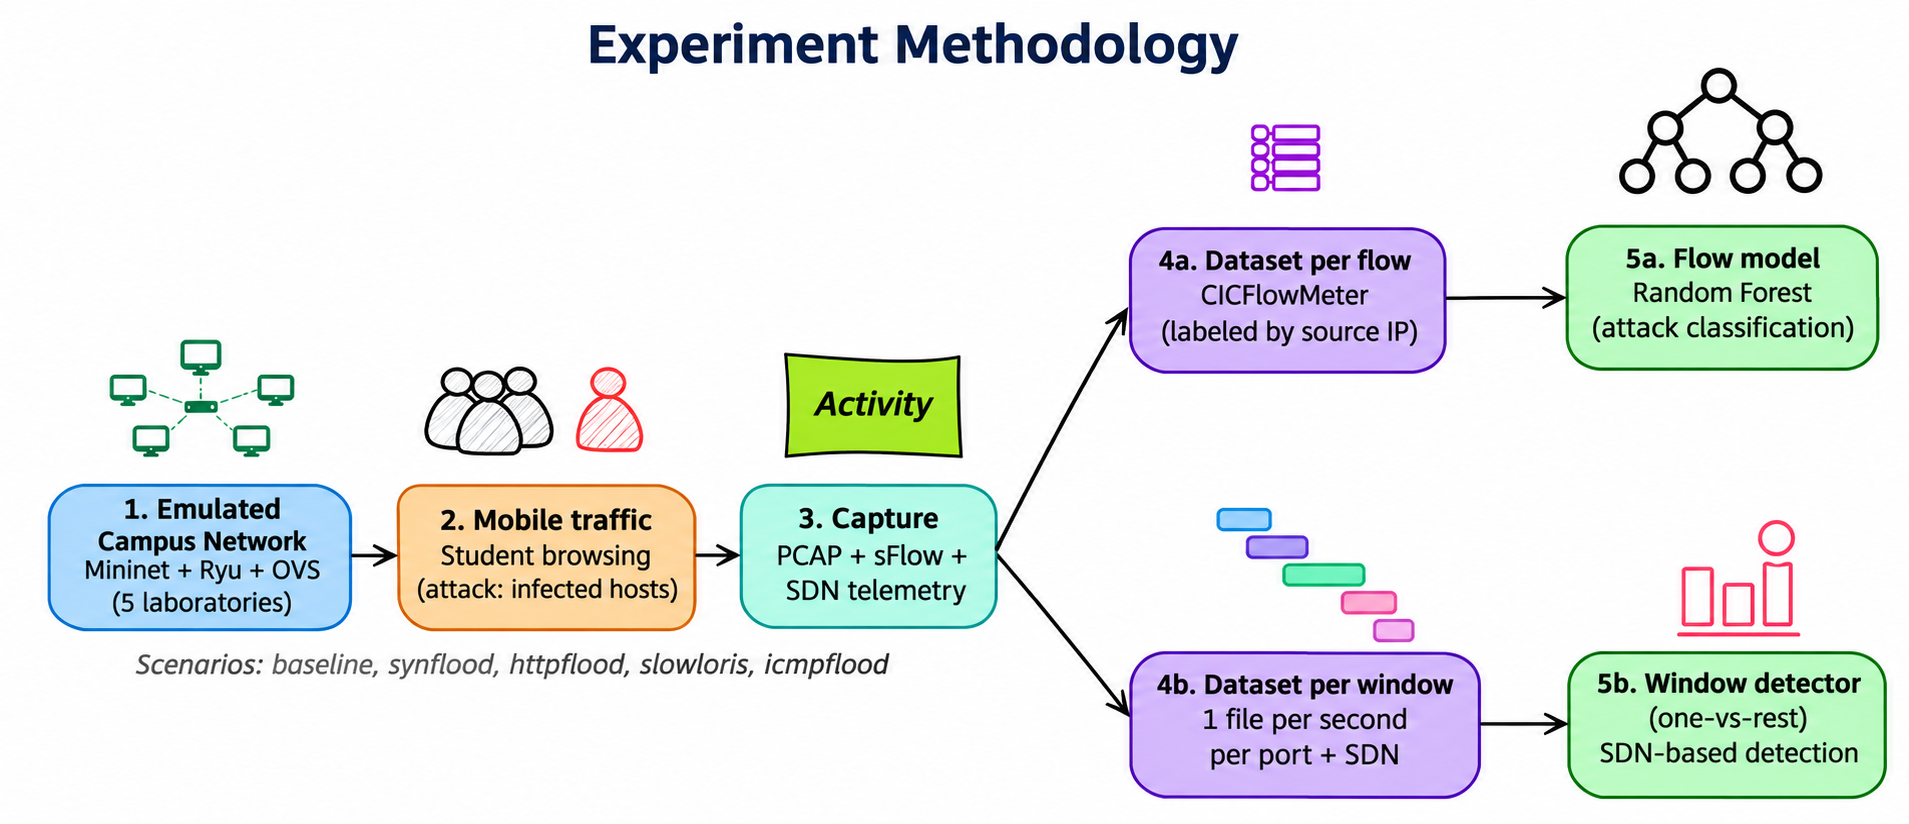
\includegraphics[width=\columnwidth]{methodology.png}
        \captionof{figure} {Experimental pipeline from the emulated campus to the model. The label comes from the sender, not the capture file.}\label{fig:methodology}
    \end{center}

  \subsection{Topology and Population}

  The topology replicates a small campus network: an edge modem, a \emph{core} switch, a DMZ hosting the web portal (the victim, \texttt{10.0.0.10}), and one lab per academic department, connected by seven Open vSwitch switches managed by Ryu. Each lab has four students and two compromised PCs (20 students and 10 infected PCs in total). The command center (C2) is located on the Internet side of the modem (\texttt{192.168.9.10}); the entire campus resides in \texttt{10.0.0.0/8}. During an attack, students continue to request pages from the portal, and the operator’s browser connects as just another benign client (\texttt{http://127.0.0.1:8080/} $\rightarrow$ \texttt{10.9.0.1}). The attack does not leave the container.

  \begin{figure*}[t]
      \centering
      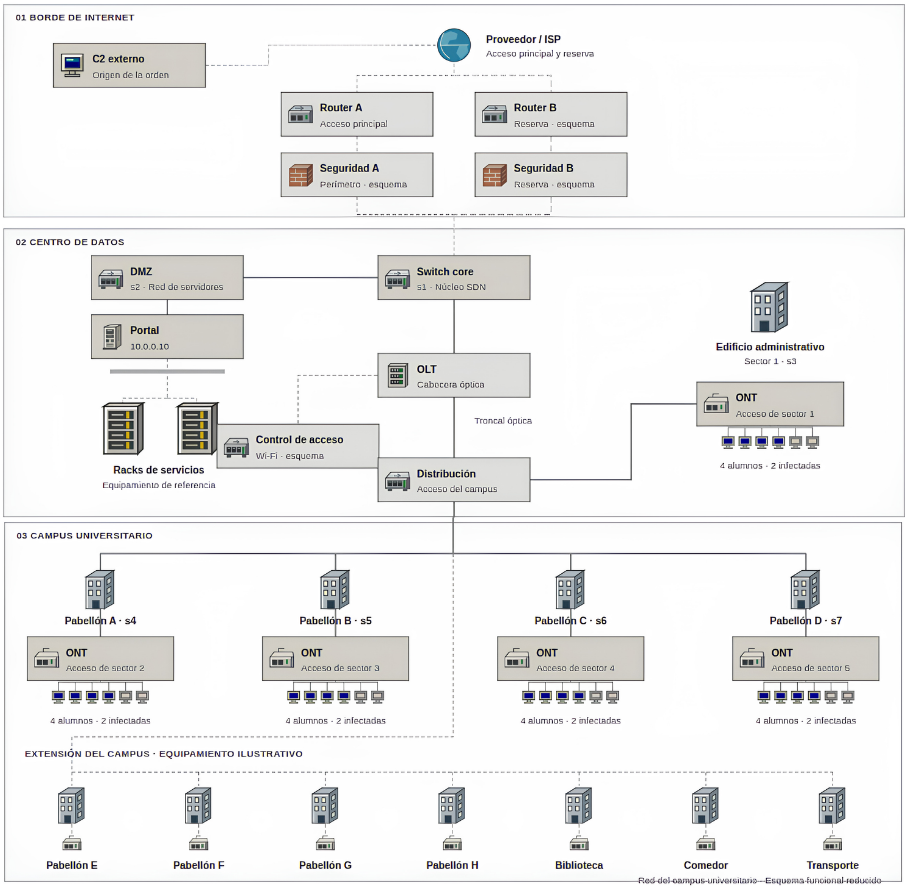
\includegraphics[width=\textwidth]{topology.png} \caption{Actual topology of the public university. For the study, the sections “02 DATA CENTER” and “03 UNIVERSITY CAMPUS” were considered. The model accounts for the addition of PCs in each building belonging to students who browse the web normally (4 per building), as well as infected PCs (2 per building) that simulate DDoS attacks against the institutional portal.}
      
      \label{fig:topology}
\end{figure*}


  \subsection{Mixed Traffic Generation}

  Compromised PCs launch one of four attack vectors: TCP-SYN flood (\texttt{hping3}), HTTP flood, Slowloris (\texttt{slowhttptest}), and ICMP flood. Sustained floods (SYN and ICMP) run in a loop with a \texttt{timeout} that restarts the generator every 5~s to maintain a consistent rate; the ICMP flood uses the kernel’s \texttt{ping}, which maintains the rate better than the \texttt{--icmp} mode of \texttt{hping3} over Open vSwitch. Since legitimate traffic never stops, each capture mixes benign and malicious flows against the same portal. The bank is orchestrated by \texttt{scripts/docker/run\_scenario.sh}, which runs one scenario or all five.

  \subsection{Capture and Measurement}

  In addition to the \texttt{pcap} captured at the portal interface, each scenario generates three synchronized data streams per second: a student probe (HTTP code, latency, and packets per second as perceived by the portal), OpenFlow controller telemetry, and container resource usage (CPU, memory, and network) via \texttt{docker stats}. The SDN telemetry is generated by a custom Ryu application (\texttt{flow\_monitor\_13.py}) which, in addition to forwarding traffic, establishes a flow for each triplet (source IP, destination IP, protocol) and periodically samples the counters for those flows on the switch (packets, bytes, and active entries). The counters are read from the switch’s data plane so that they reflect the actual volume even under sustained flooding—a necessary condition to ensure that the protocol signal (particularly ICMP) is not lost in the telemetry.

  \subsection{Tagged by Source IP}
  The fundamental truth is assigned by sender, not by capture file. A flow is \texttt{BENIGN} unless its source IP is a compromised PC and the scenario is not the \texttt{baseline}; in that case, it is named after the attack. Thus, the student, the portal, and the entire \texttt{baseline} remain \texttt{BENIGN} even within an attack capture. The compromised IP addresses are listed in the JSON file that accompanies each \texttt{pcap}.

  \subsection{Two datasets, two tasks}

  Two complementary data sets are derived from the captured traffic. \emph{By flow} (\texttt{pcap\_to\_csv.py}): TCP and UDP traffic passes through CICFlowMeter, which produces bidirectional statistics; ICMP, which does not pass through that filter, is grouped by a dedicated aggregator every 10~s (without this cutoff, each PC would leave a single, extremely long flow, and the class would end up with very few rows). Columns \texttt{sdn\_*}, derived from OpenFlow telemetry and cross-referenced by source IP, are added to each flow. Before training, the source IP, destination IP, ports, and timestamp are discarded so that the model learns behavior rather than machine identity; infinite or empty values are set to zero, and all constant columns are removed. The model is a forest of 200 trees with class-based weights, because SYN floods dominate the dataset. \emph{By time window} (\texttt{build\_windows.py}): one row per second that aggregates the portal counters and SDN telemetry for the interval (source IP entropy, traffic concentration, flow table growth, and packets per protocol), for detection \emph{while the attack is occurring}.

  \subsection(Evaluation Protocol)

  A random partition is never used, because windows and neighboring flows are correlated. The per-stream model (\texttt{analisis\_completo.py}) is evaluated using a laboratory \emph{holdout} set: four academic areas (185,127 streams) are used for training, and the model is tested on an unseen area, Agricultural Sciences (45,550 streams). The window-based detector is evaluated using \emph{leave-one-run-out} cross-validation when there are two or more runs. To obtain the mean and standard deviation, the test suite runs \texttt{run\_scenario.sh repeat N} or \texttt{dificil N}, which repeat the scenarios with different seeds and intensities (recorded in the \texttt{meta.json} file for each run). The flow-based classifier uses five 120~s runs per scenario; the window-based detector uses 20 runs that combine five intensity profiles (normal, low, stealth, pulses, and ramp), plus four never-before-seen attacks reserved solely for testing.

  \subsection{Software and Hardware requirements}

  The database runs on an Ubuntu 24.04 container; the table versions were read from the \texttt{ataque-sdn} image. The models are trained by running the analysis scripts (they are not pre-trained models): the reported detector was obtained using Python 3.10.12, scikit-learn 0.23.2, pandas 1.3.5, numpy 1.21.5, and matplotlib 3.5.1. Ryu uses Python 3.9.25 in a separate virtual environment.

  \begin{center}
    \begin{table*}[!ht]%
      \caption{Testbed requirements.}\label{tbl:testbed}

      \begin{tabular*}{\textwidth}{@{\extracolsep\fill}lcccc@{\extracolsep\fill}}
      \toprule
      &\multicolumn{2}{@{}c}{\textbf{Spanned heading$^{\tnote{\bf a}}$}} & \multicolumn{2}{@{}c}{\textbf{Spanned heading$^{\tnote{\bf b}}$}} \\\cmidrule{2-3}\cmidrule{4-5}
      \textbf{No.} & \textbf{Description}  & \textbf{Tool}  & {\textbf{Version}}  \\
      \midrule
              No. & Description & Tool & Version \\
              \midrule
              1 & Network emulator & Mininet & 2.3.0 \\
              2 & Virtual switch & Open vSwitch & 3.3.9 \\
              3 & SDN controller & Ryu & 4.34 \\
              4 & SYN and ICMP flooding & hping3 & 3.0.0-alpha-2 \\
              5 & Low-rate attack & slowhttptest & 1.9.0 \\
              6 & Packet capture & tcpdump & 4.99.4 \\
              7 & pcap to CSV & CICFlowMeter & 0.5.0 \\
              8 & Container system & Ubuntu & 24.04 \\
      \bottomrule
      \end{tabular*}
    \end{table*}
  \end{center}

  To replicate the execution, all you need is a standard desktop computer with 8 cores and 16~GB of RAM. Docker Desktop can be installed on Windows 11 or Ubuntu. The container is allocated 6 CPUs and 8~GB, and runs Ubuntu 24.04. Open vSwitch uses the kernel \emph{datapath} when the \texttt{openvswitch} module is available on the host, and automatically falls back to the userspace \emph{datapath} (\texttt{netdev}) otherwise; the flow telemetry correctly reflects sustained floods in both modes.

\section{Results and impact overview}\label{sec:impact}
The benchmark is fully reproducible: it is repeated using controlled seeds, mixing student and attack data in the same run, and produces two complementary detection pipelines. The flow-based classifier achieves a macro F1 score of \Fmacro in the Agricultural Sciences laboratory, retained from training. The window-based detector, evaluated using leave-one-run-out on 20 runs covering five intensity profiles, achieves a macro F1 score of 0{,}918~$\pm$~0{,}149. With institutional authorization, the same pipeline can process real benign traffic (Wireshark) without removing the attack from the container.

  \subsection{Dataset composition}

  The CSV files from the five runs total 230,692 flows: 143,133 \texttt{synflood}, 46,728 \texttt{BENIGN}, 36,595 \texttt{httpflood}, 3,598 \texttt{slowloris}, and 638 \texttt{icmpflood}. This distribution explains the decision to weight the classes during training; unlike in previous runs, the ICMP class now has enough flows (129 in the held-out dataset) to be meaningful. In addition, the attack captures retain a benign portion, corresponding to students who continue to use the portal.


  \subsection{Portal impact}
  \begin{table}[t]
\centering
\small
\caption{Portal probe. Each scenario lasts 120~s.}
\label{tbl:sonda}
\setlength{\tabcolsep}{4pt}
\begin{tabular}{@{}lrrrr@{}}
\toprule
Scenario & HTTP 200 & Failures & Latency (ms) & Packets/s \\
\midrule
baseline & 120 & 0 & 407 & 111 \\
synflood & 120 & 0 & 404 & 466 \\
httpflood & 120 & 0 & 564 & 386 \\
slowloris & 1 & 117 & 403 & 86 \\
icmpflood & 120 & 0 & 404 & 271 \\
\bottomrule
\end{tabular}
\end{table}



  SYN produces the highest rate, 466 packets/s, yet the probe keeps 120 HTTP 200 responses. HTTP flood raises mean latency from 407 to 564~ms. Slowloris produces only 86 packets/s but occupies available connections and fails 117 of 118 probes. Packet rate alone therefore does not describe application impact.

  \subsection{Classifier performance}
  \begin{table}[t]
\centering
\small
\caption{Detection (random forest) on the held-out Agrarias laboratory. Macro F1 \Fmacro.}
\label{tbl:deteccion}
\begin{tabular}{@{}lrrrrp{2.4cm}@{}}
\toprule
Class & Prec. & Recall & F1 & Flows & Comment \\
\midrule
BENIGN & 0.956 & 0.949 & 0.953 & 1775 & well separated \\
httpflood & 0.939 & 0.947 & 0.943 & 1458 & well separated \\
icmpflood & 1.000 & 1.000 & 1.000 & 24 & too few flows to claim \\
slowloris & 1.000 & 1.000 & 1.000 & 126 & well separated \\
synflood & 1.000 & 1.000 & 1.000 & 4708 & well separated \\
\bottomrule
\end{tabular}
\end{table}


  The F1 macro in Agrarias is \Fmacro and the binary F1 for \texttt{BENIGN} against attack is 1{,}000. Among the most influential variables are both CICFlowMeter statistics (the mean and variability of the outbound packet length and the mean outbound segment size) and columns derived from OpenFlow telemetry cross-referenced by source IP (\texttt{sdn\_avg\_pkt\_bytes}, \texttt{sdn\_bytes}, \texttt{sdn\_pkts}). This is consistent with the scenarios—SYN generates small, repeated segments, HTTP exchanges complete requests and responses, and Slowloris maintains connections with low traffic—and shows that SDN signals also provide insights at the individual flow level.


  \subsection{Early Detection Based on a Time Window}

  The per-window dataset contains 11,698 one-second windows, distributed across 20 runs that combine five intensity profiles (normal, low, stealth, pulses, and ramp). BENIGN comprises 5,175 windows, and each attack vector ranges from 1,573 to 1,652 (Fig.~\ref{fig:windows_class}). To measure generalization, the dataset also reserves four never-before-seen attacks—\texttt{ackflood}, \texttt{udpflood}, \texttt{slowpost}, and \texttt{multivector}—that only appear during testing. Each scenario lasts 120~s per run.

  \begin{center}
      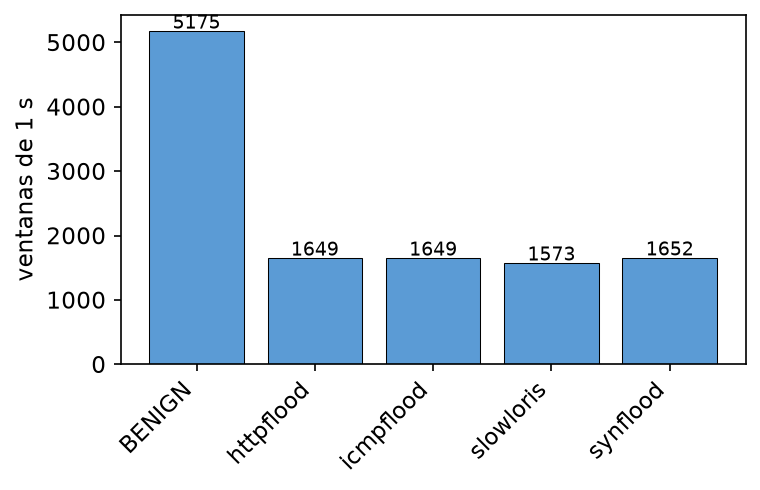
\includegraphics[width=\columnwidth]{ventanas_por_clase.png}
      \captionof{figure}{Distribution of Windows by Class in the Early Detection Dataset.}\label{fig:windows_class}
\end{center}

  Fig.~\ref{fig:packets_scenario} shows the distribution of the packet rate to the portal per second across all runs. Synflood exhibits the highest and most consistent rate. Httpflood has a lower median but with extreme outliers, reflecting the variability in intensity across runs. Slowloris is the most striking: its median is low, similar to the baseline, but it exhibits high outliers; this is consistent with its nature as a connection-exhaustion attack, rather than a volume-based attack. This dispersion confirms that packet rate alone is not sufficient to distinguish all attacks, which justifies the use of combined network, portal, and SDN telemetry features.

    \begin{center}
      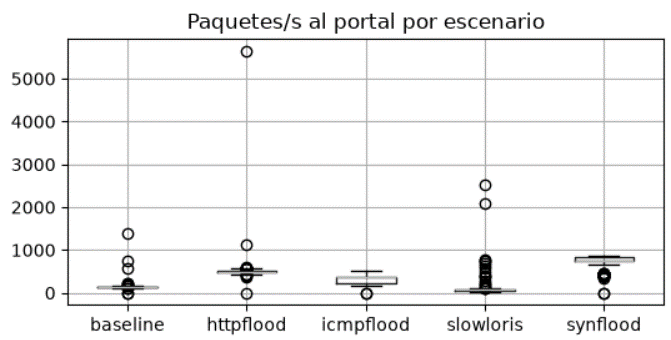
\includegraphics[width=\columnwidth]{paquetes_escenario.png}
      \captionof{figure}{Packets per second to the portal, by scenario. Slowloris and baseline traffic may be indistinguishable in terms of volume.}\label{fig:packets_scenario}
    \end{center}

  \begin{center}
        \small
        \captionof{table}{Model Comparison (leave-one-run-out, 20 folds).}
        \label{tbl:model_comparison}
        \begin{tabular}{lcccc}
              \hline
              Model & Macro F1 & $\pm$ & F1 bin. & $\pm$ \\
              \hline
              Random Forest     & 0{,}918 & 0{,}149 & 0{,}942 & 0{,}107 \\
              Gradient boosting    & 0{,}918 & 0{,}143 & 0{,}944 & 0{,}096 \\
              Logistic Regression     & 0{,}901 & 0{,}183 & 0{,}896 & 0{,}194 \\
              \hline
        \end{tabular}
  \end{center}

  Table~\ref{tbl:model_comparison} compares the three evaluated models. All three meet the working hypothesis (F1 score $>$ 0{.}90), this time on a much more demanding dataset that includes stealthy and low-intensity attack profiles. Random Forest and Gradient Boosting are equivalent; logistic regression, being a linear model, shows greater variance between runs but remains competitive. Random Forest is selected for its stability and its ability to produce interpretable feature importance scores.

  \begin{center}
      \small
      \captionof{table}{Feature ablation (random forest).}
      \label{tbl:ablacion}
      \begin{tabular}{lcc}
            \hline
            Group & Macro F1 & $\pm$ \\
            \hline
            Network only (8 features)   & 0{,}826 & 0{,}201 \\
            SDN only (20 features)  & 0{,}810 & 0{,}224 \\
            All (28 features)     & 0{,}918 & 0{,}149 \\
            \hline
      \end{tabular}
  \end{center}

  Table~\ref{tbl:ablacion} and Fig.~\ref{fig:ablacion} show feature ablation. Network features alone achieve an F1 score of 0{,}826 ($\pm$0{,}201), and SDN features alone achieve an F1 score of 0{,}810 ($\pm$0{,}224); both show high variability across folds because stealthy profiles are difficult to separate using a single set of signals. Combining both sets raises the F1 score to 0.918 ($\pm$0.149). OpenFlow telemetry contributes $+$0.092 to the macro F1 score compared to using only network counters, demonstrating that signals from the SDN controller play a complementary role in detection.

  \begin{center}
      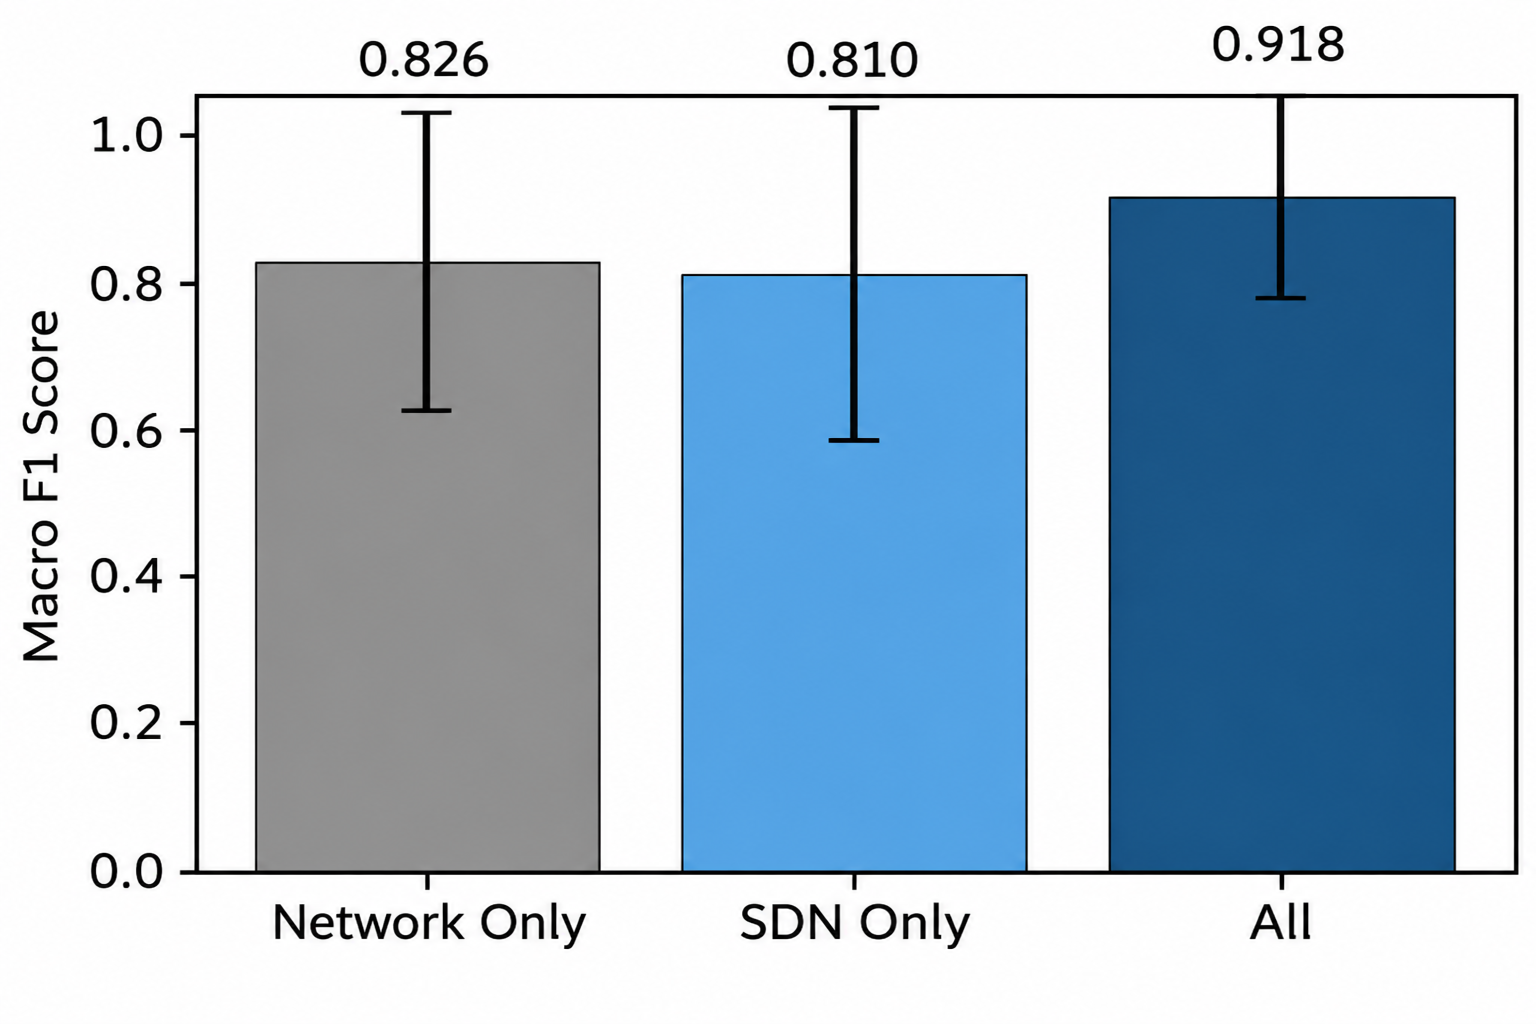
\includegraphics[width=\columnwidth]{ablacion_features_en.png}
      \captionof{figure}{Feature ablation: network, SDN, and all. The error bars indicate the standard deviation across folds.}
      \label{fig:ablacion}
  \end{center}

  \begin{center}
        \small
        \captionof{table}{Recall by class for the random forest (all features).}
        \label{tbl:recall}
        \begin{tabular}{lcc}
              \hline
              Class & Recall & $\pm$ \\
              \hline
              BENIGN     & 0{,}975 & 0{,}067 \\
              httpflood  & 0{,}856 & 0{,}291 \\
              icmpflood  & 0{,}984 & 0{,}044 \\
              slowloris  & 0{,}966 & 0{,}079 \\
              synflood   & 0{,}872 & 0{,}296 \\
              \hline
        \end{tabular}
  \end{center}

  Table~\ref{tbl:recall} details the recall by class. On benign traffic, false positives range from 2{,}5\%~$\pm$~6{,}7\%. The highest recall rates are for icmpflood (0{,}984) and slowloris (0{,}966); the two floods with the lowest recall rates are httpflood (0{,}856) and synflood (0{,}872), because under stealthy profiles, their signatures closely resemble benign traffic. The time to the first alarm is 0{,}2~s for icmpflood, 0{,}6~s for slowloris, 1{,}4~s for synflood, and 4{,}3~s for httpflood: even with difficult profiles, the model reacts within seconds.

  Fig.~\ref{fig:confusion} shows the cumulative confusion matrix across the 20 folds. The diagonal dominates: 706 errors out of 11\,698 windows (6{,}0\%), concentrated in synflood and httpflood windows marked as benign during the stealthy profiles.

  \begin{center}
        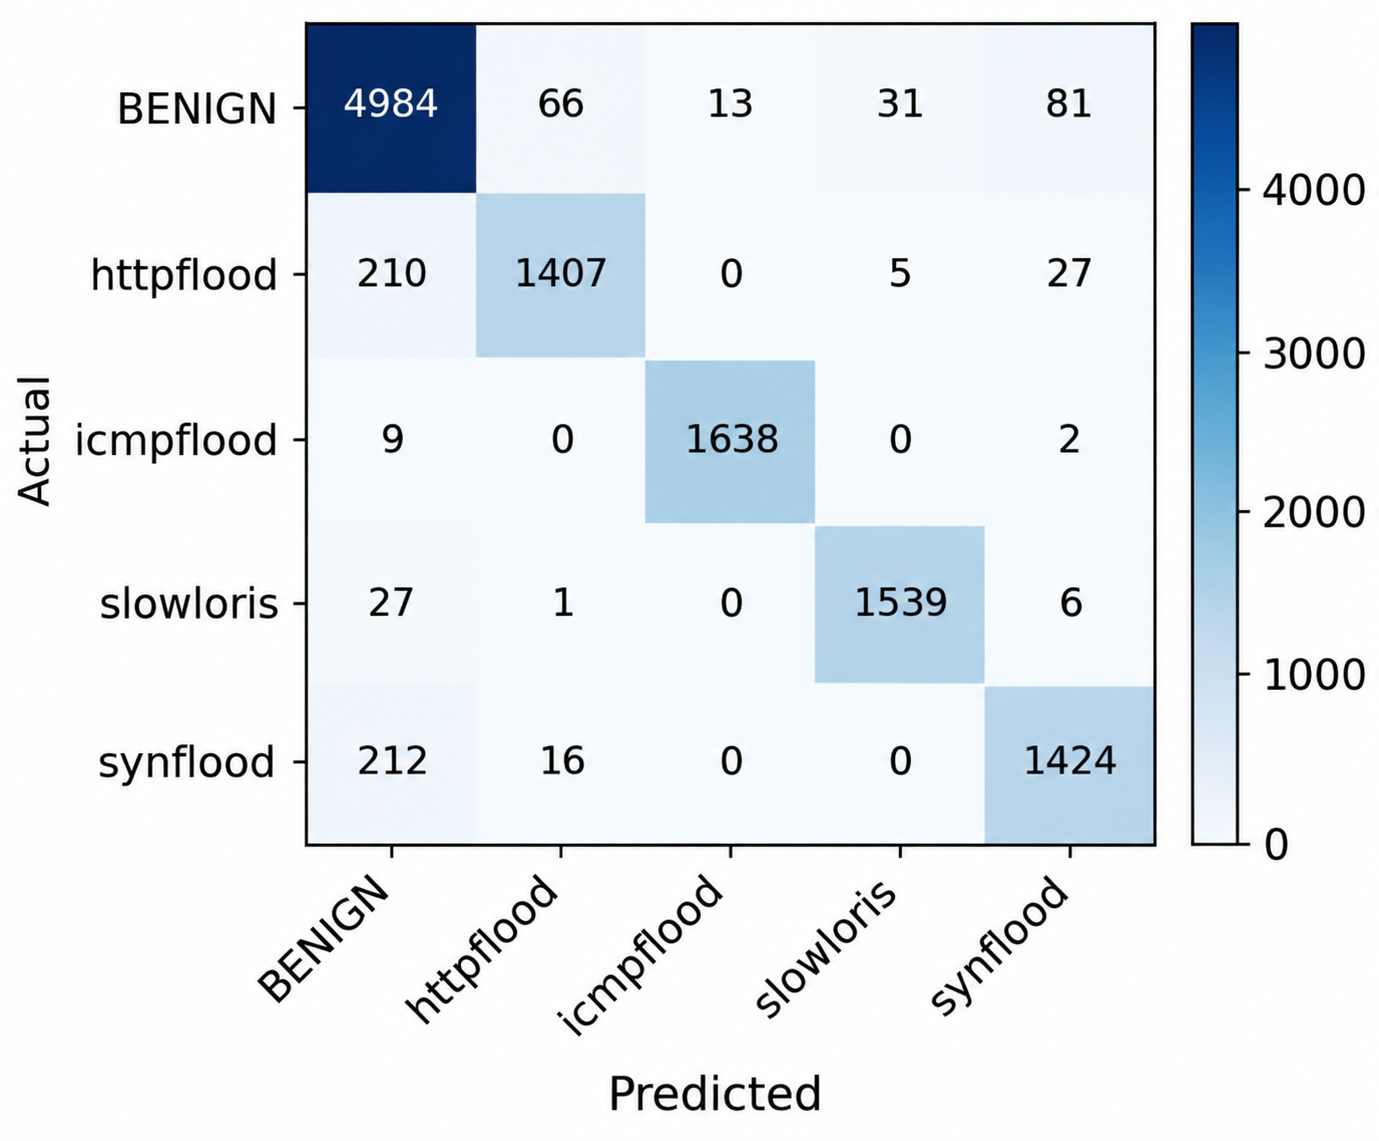
\includegraphics[width=\columnwidth]{matriz_confusion_en.png}
        \captionof{figure} {Cumulative confusion matrix across the 20 folds. Errors are concentrated in synflood and httpflood windows classified as BENIGN under the stealthy and low-intensity profiles.}
        \label{fig:confusion}
  \end{center}

  Fig.~\ref{fig:features} shows the ten features with the highest weights in the forest. The two most discriminating features are \texttt{rx\_pps\_roll3} (moving average of the packet rate to the gateway) and \texttt{conns\_roll3} (moving average of connections), followed by server metrics (\texttt{server\_rx\_pps}, \texttt{server\_conns}). Starting at the eighth position, SDN features appear (\texttt{sdn\_frac\_icmp\_roll}, \texttt{sdn\_mean\_pkts\_per\_flow}, \texttt{sdn\_pkts\_icmp}), confirming the complementary contribution of OpenFlow telemetry.

  \begin{center}
      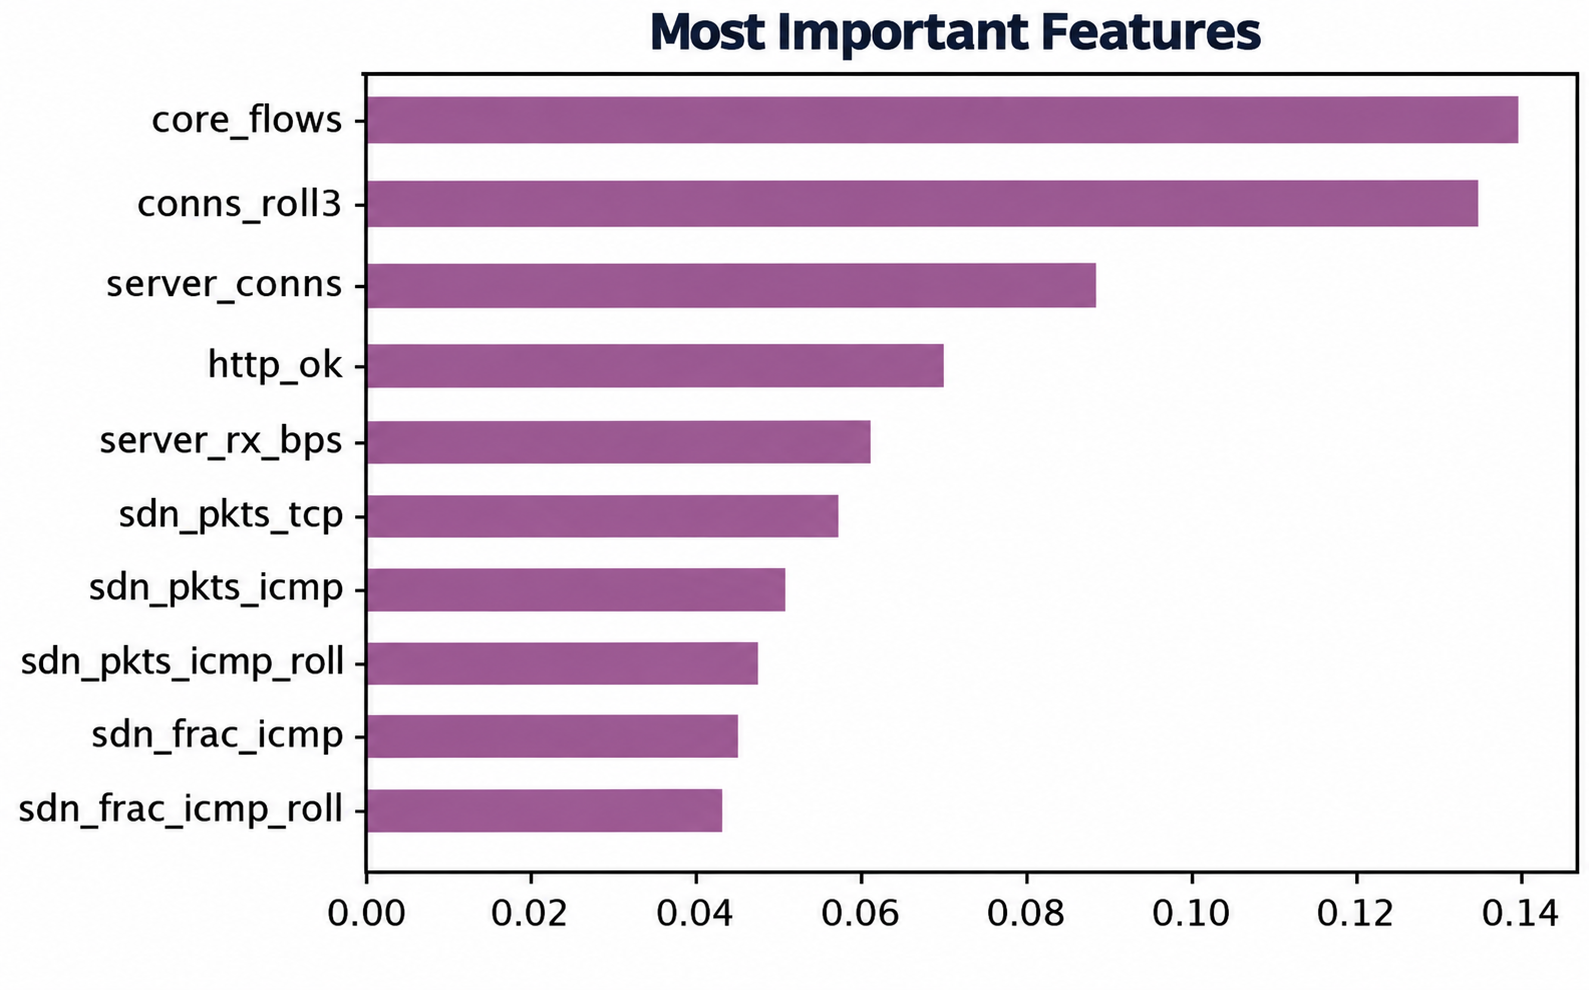
\includegraphics[width=\columnwidth]{features_importantes_en.png}
      \captionof{figure}{The ten most important features in the random forest.}
      \label{fig:features}
  \end{center}
  
  \subsection{Bank Resource Usage}

  The average CPU usage of the container was 40\% in the baseline, 36\% in SYN, 71\% in HTTP, 313\% in Slowloris, and 35\% in ICMP; in Docker, 100\% is roughly equivalent to one core. Slowloris occupied about three of the six assigned cores, while the maximum observed memory usage remained around 230~MiB (during the HTTP flood). These values measure the entire bank (Mininet, OVS, Ryu, portal, and generators), not just
  the victim.

  \subsection{Discussion}
  The test supports the hypothesis for all five classes: the model achieves a macro F1 score above 0.90 without IP and generalizes to a held-out lab. For the window-based detector, we avoid the naive interpretation of an F1 close to 1: by adding stealthy, low-intensity attack profiles—in pulses and ramps—the honest macro F1 drops to 0{,}918~$\pm$~0{,}149 (\emph{leave-one-run-out} over 20 runs). The gap between training and testing has a median per run of $-0{,}011$—the model does not memorize—and only spikes in the few runs with the stealthy profile, where the attack is nearly indistinguishable from normal traffic. The most demanding test—leaving an entire profile out of training—yields a mean macro F1 score of 0{,}742 with absolute features and 0{,}764 with relative features compared to each run’s baseline; these figures—not a value close to 1—are the defensible results. When faced with four never-before-seen attacks (\texttt{ackflood}, \texttt{udpflood}, \texttt{slowpost}, and \texttt{multivector}), the detector triggers an alarm in 97\% of the attack windows using relative features. The most informative result remains the ablation: the fact that OpenFlow telemetry contributes $+$0{,}092 to the macro F1 score and is decisive in distinguishing ICMP from SYN is concrete evidence that SDN-specific signals have discriminative value that non-SDN datasets do not offer. The difference between SYN and Slowloris also demonstrates why it is beneficial to combine flow classification with a service probe: more packets do not necessarily mean a less available page.

  \subsection{Limitations and future improvements}
  The table is still computed from emulated students. The hybrid dataset (Wireshark plus simulated attack) is ready in the code and is updated when the authorized pcaps arrive. The reported per-flow result comes from a single 120~s run; the \texttt{repeat} driver and the leave-one-run-out cross-validation now make the evaluation repeatable, and the multi-run figures (mean~$\pm$~standard deviation) are being regenerated. ICMP accounts for 120 flows in the whole set and 24 in the Agrarias test, so its perfect F1 is not reported as a settled class result. The per-window detector is designed for early detection and consumes the controller telemetry that a Ryu-side detector would use, but it still scores already-captured windows offline rather than running inside Ryu. Future work: report the multi-run cross-validated figures and the SDN ablation, repeat the test with the Wireshark background and a mixed four-vector scenario, add more ICMP samples, and move the trained per-window model into the controller for online detection.

  \section{Conclusions}
  Campus-DDoS-SDN is a reproducible, single-command testbed that does not rely on live internet connectivity and generates a multi-class DDoS dataset in which benign traffic and four attack vectors coexist in the same capture against a single portal. Source-based labeling preserves benign traffic within the attacked capture, and laboratory-based partitioning provides a more demanding test than a random split. On completed flows, a random forest trained without IPs, ports, or timestamps achieves a macro F1 score of \Fmacro in the retained Agricultural Sciences laboratory; on the window-based dataset, it enables early detection with a macro F1 score of 0{,}918 across 20 runs covering five intensity profiles (and up to 0{,}764 when leaving an entire profile out of training), where OpenFlow telemetry contributes $+$0{,}092 and proves decisive in separating ICMP from SYN. This confirms the central contribution of the study: SDN-specific signals, absent from reused non-SDN datasets, have measurable discriminatory value.

  Availability, packet rate, and classification describe different aspects of the incident: only Slowloris takes the portal offline despite its low packet rate. The result, using emulated students, serves as the basis for requesting authorization to incorporate real benign traffic from UNCP, without removing the attack from the container.

\section*{Acknowledgements}
The authors thank the Universidad Nacional del Centro del Per\'u.

\bibliography{references.bib}

\end{document}
